\section{Introduction}
  \label{sec:introduction}
  Genetic algorithms (GAs) are a typical approach in evolutionary computation and are a representative meta-heuristic approach. The key operators of the GA are selection, crossover, mutation, and replacement. By properly organizing the operators, the performance of GA can be moderated. Therefore, proper tuning of GA parameters can be considered as the most important part in building a GA. \\
  There has been much research on parameter optimization. Research that attempted to automate GA tuning using meta-genetic algorithms has been very popular following the first attempt by Grefenstette~\cite{grefenstette1986optimization}. There was also an early attempt similar to Grefenstette's using meta-GA. Lee and Takagi~\cite{lee1993integrating} used the GA and penalty strategies and proposed a method to design an automated fuzzy system. Until recently, research on parameter optimization using meta-GA was actively conducted. \\
  As in this paper, there has been research using machine learning in GA parameter optimization. Cooray and Rupasinghe~\cite{cooray2017machine} used machine learning to solve the energy minimizing vehicle routing problem. They bundled the data using $k$-means clustering method, and they categorized data based on basic characteristics. The GA parameters were chosen based on the various tuning methods, which resulted in outstanding performance. \\
  We intend to take a new approach in GA parameter optimization using machine learning. We would like to apply our approach to the $NK$-landscape problem. The objective of this study is to train with data consisting of a GA parameter set using support vector regression (SVR) and an approximate GA parameter space. In addition, based on the approximation results, we intend to analyze the GA parameter space.


\section{Parameter Space of GA \& SVR Approximation}
  \label{sec:parameter-svr}
  \subsection{Parameters of GA}
    \label{sec:parameters-ga}
    The GA parameters are presented in this section. The relevant GA parameters are selection, crossover, mutation, and replacement. Moreover, tuning parameters of GA can be seen as moderating these operators. The parameters to be covered in this research are as follows. \\
    $\bullet$~\textbf{Population size:} the population size was a randomly generated number between $10$ and $5,000$. \\
    $\bullet$~\textbf{Selection type:} when moving from the existing generation to the next generation, one has to choose a population. Four selection methods were used---roulette wheel selection, scaled roulette wheel selection, tournament selection, and rank-based selection. \\
    $\bullet$~\textbf{Crossover type:} we used $n$-point crossover and uniform crossover. Moreover, when using $n$-point crossover, the number of points ranged from $1$ to $5$. \\
    $\bullet$~\textbf{Mutation rate:} the mutation rate ranged from $0$ to $0.25$, and random numbers were generated and used per $0.001$ unit. \\
    $\bullet$~\textbf{Replacement type:} we used 4 methods, which were replacement of the worst individuals in the population, replacement of similar individuals in the population, replacement of worst individuals among the parents, and the replacement of similar individuals among the parents.

  \subsection{SVR Approximation}
    \label{sec:svr-approximation}
    SVR is a supervised learning model used to analyze regression. By using SVR, the GA parameter space was approximated as shown in Figure~\ref{fig:1}. For SVR modeling, 100 data points generated $f(x)$, and 10 arbitrarily chosen points were extracted to train $f(x)$. Using the SVR model built upon this process, we generated 100 points and approximated the original $f(x)$. Figure~\ref{fig:1-a} demonstrates a rather simple problem, and the SVR model could make up the trends of changes highly similar to the original data with just 10 data points. On the other hand, Figure~\ref{fig:1-b} illustrates rather more complex functions. The trained SVR model did not yield the best approximations of the original function.
    
    \begin{figure}[t]
      \centering
      \subcaptionbox{
        Well approximated \boldmath$f(x)$
        \label{fig:1-a}
      }{
        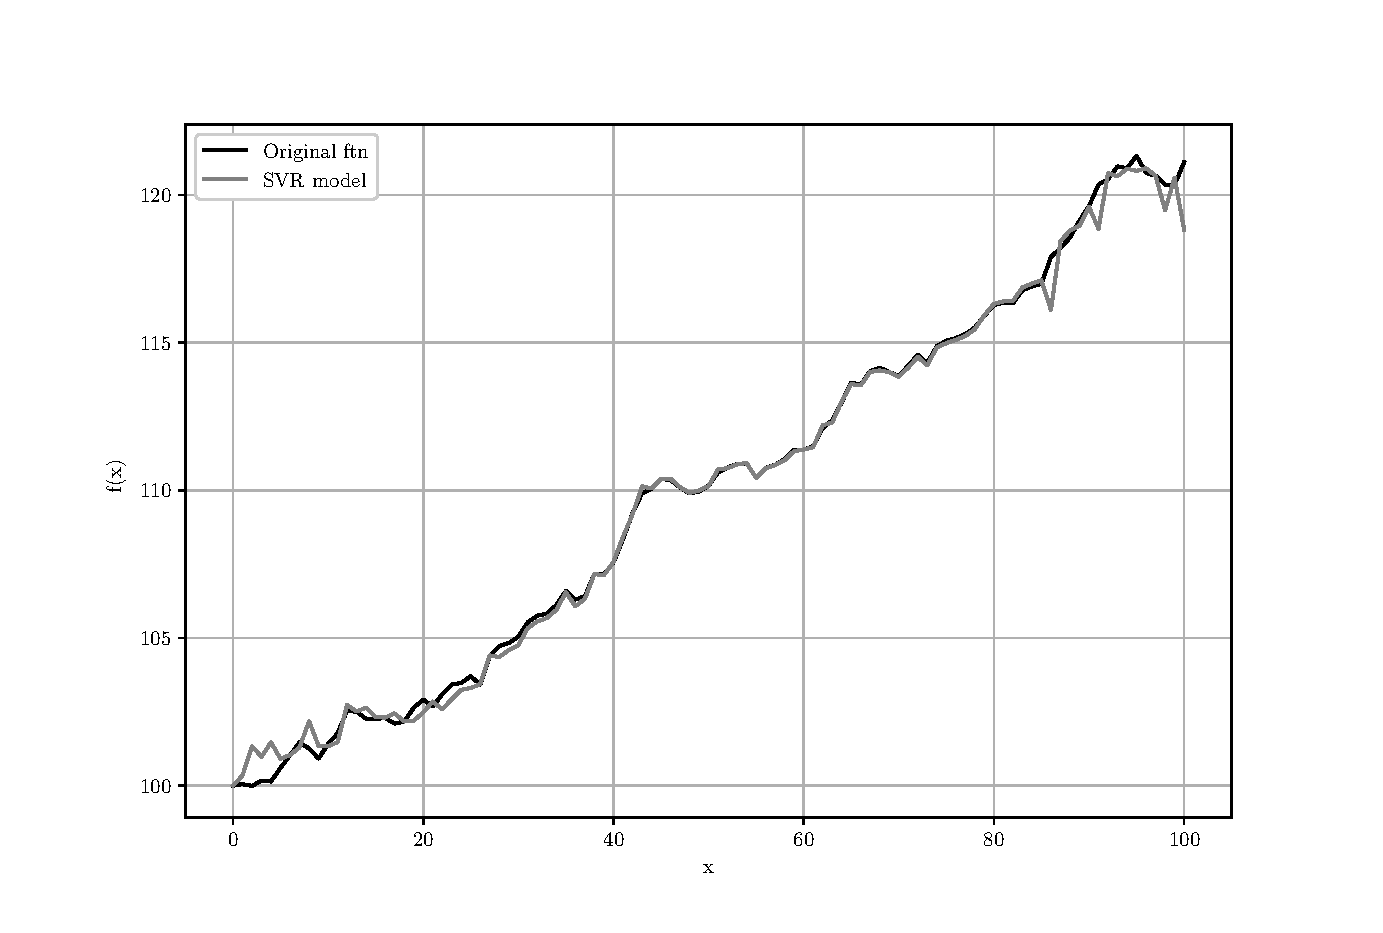
\includegraphics[width=0.45\columnwidth]{figure1-a}
      }
      \subcaptionbox{
        Badly approximated \boldmath$f(x)$
        \label{fig:1-b}
      }{
        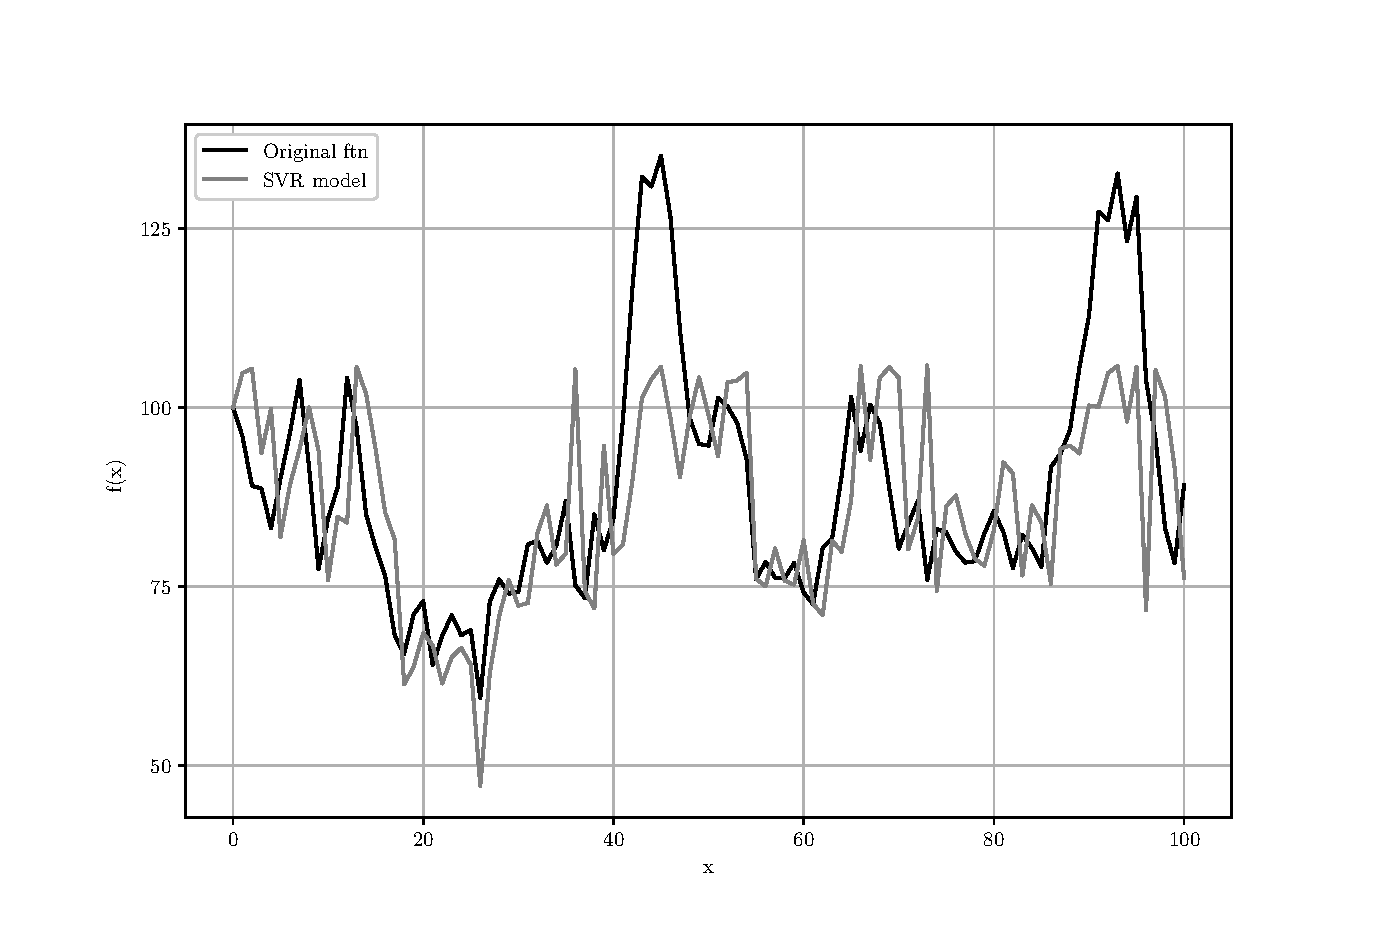
\includegraphics[width=0.45\columnwidth]{figure1-b}
      }
      \caption{Examples of function approximation by SVR}
      \label{fig:1}
    \end{figure}


\section{Results \& Analysis}
  \label{sec:results}
  The SVR model presented in Section~\ref{sec:parameter-svr} was applied to the $NK$-landscape problem. The value of $N$ in the $NK$-landscape problem was $50$, and $K$ was $4$. The fitness contribution was arbitrarily generated from real numbers ranging between $0$ and $1$. Moreover, we use steady-state GA with a generation size of $10,000$. Table~\ref{tab:1} describes the performance of $10,000$ best fitness data and SVR model according to the parameters of GA. Table~\ref{tab:2} shows the results obtained by finding $100$ optimal points of SVR model using GA*\footnote{GA{*} is a GA used to find the optimal point of the SVR model, so it is a steady-state GA with a generation size of $20,000$. The population size is $1,000$, the chromosomes of each individual are the 5 parameter values used in Section \ref{sec:parameters-ga}, which are integer encoding. This GA* uses rank-based selection, uniform crossover, one point mutation, and worst individual replacement, and searches for the optimal point in an SVR model.} and performing GA with the optimal points. The parameters of the $100$ optimal points in SVR model identified by GA{*} can be delineated as follows. The scaled roulette wheel selection method one-point crossover method, and similar individual replacement method were used. The best fitness results showed differences according to the size of population and mutation rate. The performance of the parameter set found was on average top $11.7$\%. In addition, one point was equal to $37.452$, which was the best result in $10,000$ best fitness data. Accordingly, although we could not find the parameter better than the one from $10,000$ datasets, we could arrive at a relatively proper parameter set. The mean absolute error (MAE) of the dataset from 10-fold cross-validation was approximately $0.478$. The difference between the optimal points of SVR model and actual results of GA was approximately $2.101$, which was a considerable difference. \\
  Figure ~\ref{fig:2} shows the best fitness results for 100 optimal points in the SVR model according to population size and mutation rate of GA. Figure ~\ref{fig:2-a} shows a 3D view of the best fitness over the two parameters, and Figure ~\ref{fig:2-b} presents a cross-sectional view of Figure ~\ref{fig:2-a}. \\
  As can be seen in Figure~\ref{fig:2-a}, the best fitness values are extremely vulnerable to minor changes in the parameters. From these, one can realize that the GA parameter space is structured in a complex way. As a result, due to the complexities of the GA parameter space, it is not simple to arrive at optimal GA parameters with machine learning.

  \begin{table}[t]
    \centering
    \caption{SVR model results from the 10,000 dataset}
    \label{tab:1}
    \vspace{-0.5em}
    \small
    \begin{tabu}{X[l] || X[r] X[r] X[r]}
      \toprule
      & Best & Average & SD\footnotemark \\
      \hline\hline
      Best fitness & 37.452 & 33.316 & 1.707 \\
      SVR model & 37.873 & 33.280 & 1.581 \\
      \bottomrule
    \end{tabu}
  \end{table}
  \footnotetext{Standard deviation}

  \begin{table}[t]
    \centering
    \caption{Actual GA results and 100 optimal points of model}
    \label{tab:2}
    \vspace{-0.5em}
    \small
    \begin{tabu}{X[l] || X[r] X[r] X[r]}
      \toprule
      & Best & Average & SD \\
      \hline\hline
      SVR model & 37.965 & 37.955 & 0.008 \\
      GA & 37.452 & 35.836 & 0.726 \\
      \bottomrule
    \end{tabu}
  \end{table}

  \begin{figure}[t]
      \centering
      \subcaptionbox{
        3D plot
        \label{fig:2-a}
      }{
        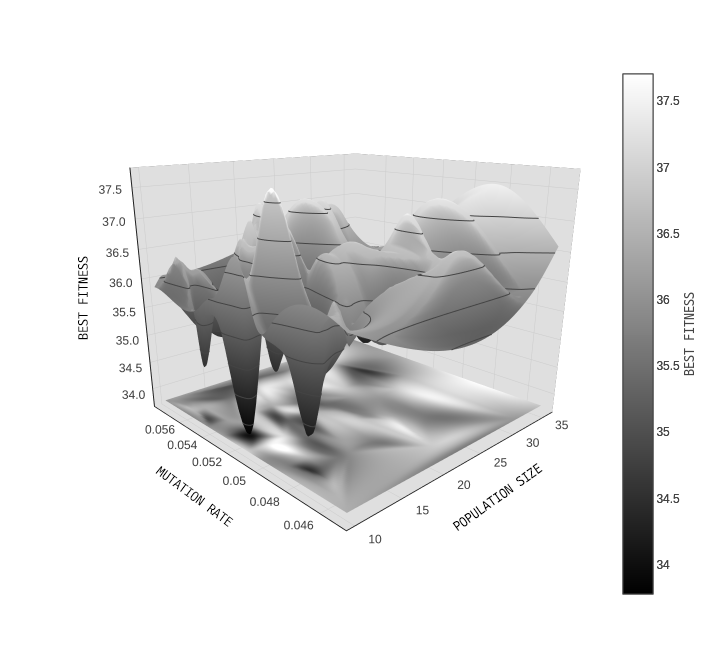
\includegraphics[width=0.45\columnwidth]{figure2-a}
      }
      \subcaptionbox{
        Contour plot
        \label{fig:2-b}
      }{
        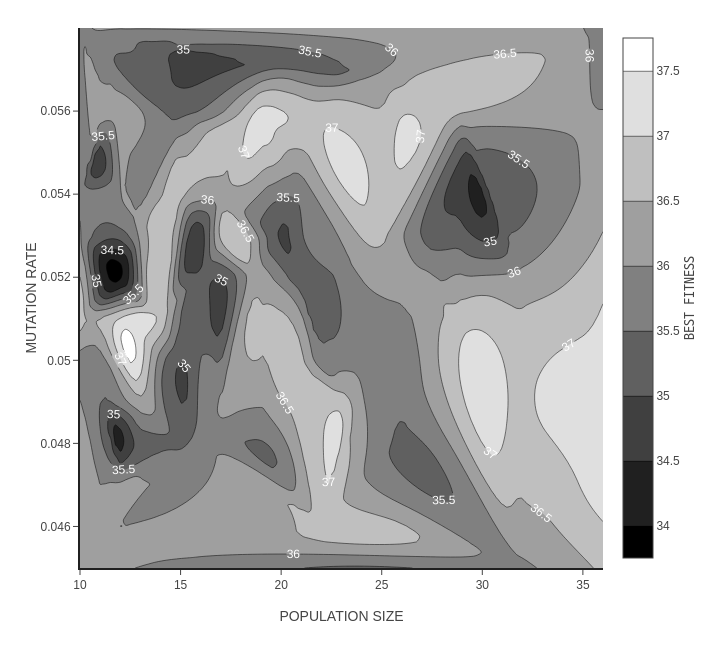
\includegraphics[width=0.45\columnwidth]{figure2-b}
      }
    \caption{GA results according to parameters (using \textit{Plotly})}
    \label{fig:2}
  \end{figure}


\section{Conclusion}
  \label{sec:conclusion}
  Machine learning has applications in various fields. Parameter optimization in GA is an important factor to determine the GA performance. In this study, we proposed an approach that applies machine learning to the GA parameter space. By using SVR, we trained the data consisting of the GA parameter set and built models. In addition, the SVR model was applied to the $NK$-landscape problem, and tried to find the optimal parameter. The identified parameter set showed performance of the top $11.7$\% on average, which can be considered as an outstanding set, but this was still not as good as the one from the dataset. As well, based on the findings from SVR approximation in the GA parameter space, GA performance is vulnerable to minor changes in the parameters. From these findings, we confirmed the challenges facing the optimization of GA parameters using machine learning. In conclusion, we could understand the complexities of the GA parameter space. The research findings will contribute to future research on GA parameter optimization.
